\section{Wireless\-Channel Class Reference}
\label{classWirelessChannel}\index{WirelessChannel@{WirelessChannel}}
Defines the channel used for radio transmissions over a wireless channel.  


{\tt \#include $<$wireless\_\-channel.hpp$>$}

Inheritance diagram for Wireless\-Channel::\begin{figure}[H]
\begin{center}
\leavevmode
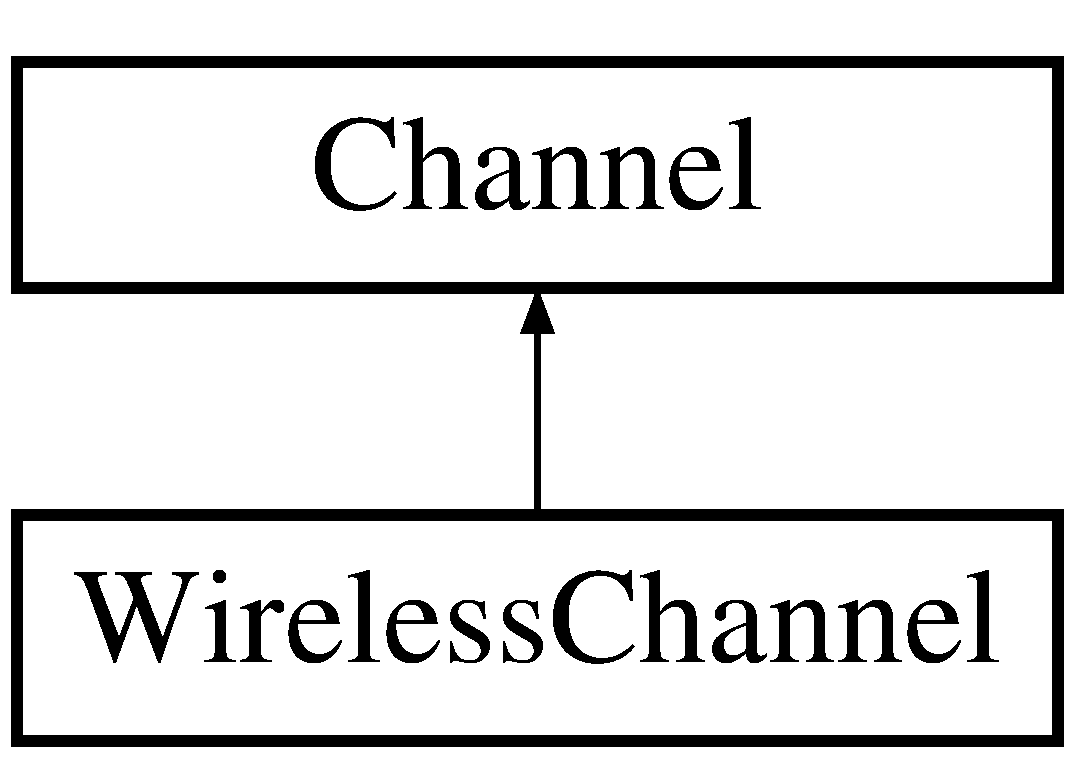
\includegraphics[height=2cm]{classWirelessChannel}
\end{center}
\end{figure}
\subsection*{Public Types}
\begin{CompactItemize}
\item 
typedef boost::shared\_\-ptr$<$ \bf{Wireless\-Channel} $>$ \bf{Wireless\-Channel\-Ptr}\label{classWirelessChannel_abd360d48a9d01c3264f4974878d334a}

\begin{CompactList}\small\item\em Smart pointer that clients should use. \item\end{CompactList}\end{CompactItemize}
\subsection*{Public Member Functions}
\begin{CompactItemize}
\item 
virtual double \bf{get\-Recvd\-Strength} (const \bf{Wireless\-Comm\-Signal} \&signal, const \bf{Physical\-Layer} \&receiver) const 
\begin{CompactList}\small\item\em Compute the signal strength at the receiver for the given signal. \item\end{CompactList}\item 
virtual bool \bf{signal\-Has\-Error} (double signal\-Sinr, const \bf{Wireless\-Comm\-Signal} \&signal) const 
\begin{CompactList}\small\item\em Computes whether or not the signal has an error each time it is called based on some channel error model. \item\end{CompactList}\end{CompactItemize}
\subsection*{Static Public Member Functions}
\begin{CompactItemize}
\item 
static \bf{Wireless\-Channel\-Ptr} \bf{create} (Path\-Loss\-Ptr path\-Loss\-Model)
\begin{CompactList}\small\item\em A factory method to ensure that all objects are created via {\tt new} since we are using smart pointers. \item\end{CompactList}\item 
static \bf{Wireless\-Channel\-Ptr} \bf{create} (Path\-Loss\-Ptr path\-Loss\-Model, Fading\-Ptr fading\-Model)
\begin{CompactList}\small\item\em A factory method to ensure that all objects are created via {\tt new} since we are using smart pointers. \item\end{CompactList}\end{CompactItemize}
\subsection*{Protected Member Functions}
\begin{CompactItemize}
\item 
\bf{Wireless\-Channel} (Path\-Loss\-Ptr path\-Loss\-Model)
\begin{CompactList}\small\item\em A constructor. \item\end{CompactList}\item 
\bf{Wireless\-Channel} (Path\-Loss\-Ptr path\-Loss\-Model, Fading\-Ptr fading\-Model)
\begin{CompactList}\small\item\em A constructor. \item\end{CompactList}\end{CompactItemize}


\subsection{Detailed Description}
Defines the channel used for radio transmissions over a wireless channel. 



Definition at line 20 of file wireless\_\-channel.hpp.

\subsection{Constructor \& Destructor Documentation}
\index{WirelessChannel@{Wireless\-Channel}!WirelessChannel@{WirelessChannel}}
\index{WirelessChannel@{WirelessChannel}!WirelessChannel@{Wireless\-Channel}}
\subsubsection{\setlength{\rightskip}{0pt plus 5cm}Wireless\-Channel::Wireless\-Channel (Path\-Loss\-Ptr {\em path\-Loss\-Model})\hspace{0.3cm}{\tt  [protected]}}\label{classWirelessChannel_7d4848d7d49d3c90883e901b710feb5a}


A constructor. 

\begin{Desc}
\item[Parameters:]
\begin{description}
\item[{\em path\-Loss\-Model}]the path loss model that the channel will use. \end{description}
\end{Desc}


Definition at line 9 of file wireless\_\-channel.cpp.

Referenced by create().\index{WirelessChannel@{Wireless\-Channel}!WirelessChannel@{WirelessChannel}}
\index{WirelessChannel@{WirelessChannel}!WirelessChannel@{Wireless\-Channel}}
\subsubsection{\setlength{\rightskip}{0pt plus 5cm}Wireless\-Channel::Wireless\-Channel (Path\-Loss\-Ptr {\em path\-Loss\-Model}, Fading\-Ptr {\em fading\-Model})\hspace{0.3cm}{\tt  [protected]}}\label{classWirelessChannel_3d6e95f3cd66299d212f42c32f6b637a}


A constructor. 

\begin{Desc}
\item[Parameters:]
\begin{description}
\item[{\em path\-Loss\-Model}]the path loss model that the channel will use. \item[{\em fading\-Model}]the fading model that the channel will use. \end{description}
\end{Desc}


Definition at line 15 of file wireless\_\-channel.cpp.

\subsection{Member Function Documentation}
\index{WirelessChannel@{Wireless\-Channel}!create@{create}}
\index{create@{create}!WirelessChannel@{Wireless\-Channel}}
\subsubsection{\setlength{\rightskip}{0pt plus 5cm}\bf{Wireless\-Channel\-Ptr} Wireless\-Channel::create (Path\-Loss\-Ptr {\em path\-Loss\-Model}, Fading\-Ptr {\em fading\-Model})\hspace{0.3cm}{\tt  [inline, static]}}\label{classWirelessChannel_8c58b20240a8a0d54c9ba5ac02f6ce3c}


A factory method to ensure that all objects are created via {\tt new} since we are using smart pointers. 

\begin{Desc}
\item[Parameters:]
\begin{description}
\item[{\em path\-Loss\-Model}]the path loss model that the channel will use. \item[{\em fading\-Model}]the fading model that the channel will use. \end{description}
\end{Desc}


Definition at line 108 of file wireless\_\-channel.hpp.

References Wireless\-Channel().\index{WirelessChannel@{Wireless\-Channel}!create@{create}}
\index{create@{create}!WirelessChannel@{Wireless\-Channel}}
\subsubsection{\setlength{\rightskip}{0pt plus 5cm}\bf{Wireless\-Channel\-Ptr} Wireless\-Channel::create (Path\-Loss\-Ptr {\em path\-Loss\-Model})\hspace{0.3cm}{\tt  [inline, static]}}\label{classWirelessChannel_111126e58d9d50d8e262bd1721b495e4}


A factory method to ensure that all objects are created via {\tt new} since we are using smart pointers. 

\begin{Desc}
\item[Parameters:]
\begin{description}
\item[{\em path\-Loss\-Model}]the path loss model that the channel will use. \end{description}
\end{Desc}


Definition at line 101 of file wireless\_\-channel.hpp.

References Wireless\-Channel().\index{WirelessChannel@{Wireless\-Channel}!getRecvdStrength@{getRecvdStrength}}
\index{getRecvdStrength@{getRecvdStrength}!WirelessChannel@{Wireless\-Channel}}
\subsubsection{\setlength{\rightskip}{0pt plus 5cm}double Wireless\-Channel::get\-Recvd\-Strength (const \bf{Wireless\-Comm\-Signal} \& {\em signal}, const \bf{Physical\-Layer} \& {\em receiver}) const\hspace{0.3cm}{\tt  [virtual]}}\label{classWirelessChannel_962a8c978b3ba7f86d5e4c6c06b4c2cf}


Compute the signal strength at the receiver for the given signal. 

\begin{Desc}
\item[Parameters:]
\begin{description}
\item[{\em signal}]the signal being transmitted. \item[{\em receiver}]the physical layer object for which we will compute the received signal strength. \end{description}
\end{Desc}
\begin{Desc}
\item[Returns:]the received signal strength value. \end{Desc}


Definition at line 24 of file wireless\_\-channel.cpp.

References Communication\-Layer::get\-Node\-Id(), Log\-Stream\-Manager::instance(), and Log\-Stream\-Manager::log\-Debug\-Item().\index{WirelessChannel@{Wireless\-Channel}!signalHasError@{signalHasError}}
\index{signalHasError@{signalHasError}!WirelessChannel@{Wireless\-Channel}}
\subsubsection{\setlength{\rightskip}{0pt plus 5cm}bool Wireless\-Channel::signal\-Has\-Error (double {\em signal\-Sinr}, const \bf{Wireless\-Comm\-Signal} \& {\em signal}) const\hspace{0.3cm}{\tt  [virtual]}}\label{classWirelessChannel_ddd5107833915f0997864a635b34fc5c}


Computes whether or not the signal has an error each time it is called based on some channel error model. 

In general, a signal's error rate is based on its SINR, length, and data rate. The SINR is given as a parameter and the other two factors are included in the signal's packet. \begin{Desc}
\item[Parameters:]
\begin{description}
\item[{\em signal\-Sinr}]the current SINR of the signal. \item[{\em signal}]the signal being tested, which includes the length and data rate of the signal's packet. \end{description}
\end{Desc}
\begin{Desc}
\item[Returns:]true if an error occurs in the signal. \end{Desc}


Definition at line 50 of file wireless\_\-channel.cpp.

The documentation for this class was generated from the following files:\begin{CompactItemize}
\item 
wireless\_\-channel.hpp\item 
wireless\_\-channel.cpp\end{CompactItemize}
